\section{Kalman-Filter \dcsecondauthorshort}
\label{sec:fahrspurerkennung_kalman}
Auch die folgende Vorgehensweise zur Fahrspurerkennung approximiert den Verlauf der Straße als Polynom 3. Grades. Durch Veränderungen abseits dieser zentralen Komponente sollten jedoch Schwächen des 1. Ansatzes zur Erkennung der Fahrbahnmarkierungen behoben werden:
\begin{itemize}
\item Mittels eines prinzipbedingt als konstant angenommenen Abstand der rechten, mittleren und linken Linie sollte ein \glqq Ineinanderlaufen\grqq{} der \gls{acr:roi}
%\footnote{Die \gls{acr:roi} stellen in diesem Fall die senkrecht zum Polynom aufgestellten Scanlines dar.} 
zur Erkennung selbiger verhindert werden. Hierfür wird nicht mehr jede Fahrspurmarkierung einzeln, sondern nur noch die Mittellinie modelliert. Um die seitlichen Linien zu erhalten, kann dieser Verlauf verschoben werden.
\item Das in Abschnitt~\ref{sec:grundlagen:kalman-filter} eingeführte Kalman-Filter soll verwendet werden, um die Lage der Fahrbahnmarkierungen in konsekutiven Aufnahmen zu verfolgen und somit zuverlässigere \gls{acr:roi} Zur Erkennung der Linien aufzuspannen.
\item Da nur kleine Teile des Bildes mit einem Kantendetektor bearbeitet werden und keine Binarisierung der Filterantwort stattfinden muss, sollte der Algorithmus schneller ablaufen können.
\end{itemize}
Final sollen die in Einzelbildern erkannten, mittig auf der Straßenmarkierung liegenden Punkte in die Weltkarte eingetragen und somit für den Regelungsalgorithmus verfügbar gemacht werden. Abbildung \ref{fig:kalman:iteration_komplett} vermittelt eine erste Idee der im Folgenden genauer beschriebenen Methode.

\begin{figure}[htbp]
\centering
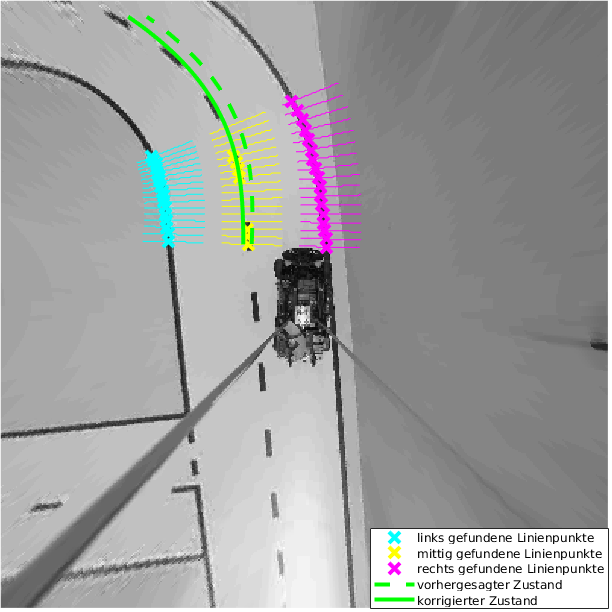
\includegraphics[width=0.75\textwidth]{kalman_iteration_komplett}
\caption{Plot einer Iteration des Kalmanfilters}
\label{fig:kalman:iteration_komplett}
\end{figure}
 
\subsection{Fahrspurmodell}
Als Repräsentation der Fahrspur im Zustandsraum soll das in \autocite{petersfalkoFPGAbasierteBildverarbeitungspipelineZur2009} vorgeschlagene Modell, welches wiederum eine Vereinfachung von \autocite{risackRobustLaneRecognition1998} darstellt, verwendet werden.
Wie in bereits angekündigt, wird die Fahrspur als Polynom 3. Grades \begin{math} \gls{y}^{\gls{lat:LinienKOS}}(\gls{x}^{\gls{lat:LinienKOS}}) \end{math} approximiert. Um die \glsdesc{lat:systemmatrix} \gls{lat:systemmatrix} zu vereinfachen und einen sehr anschaulichen \glsdesc{lat:statevector} \gls{lat:statevector} zu erhalten, wird für jenen die 0. bis 3. Ableitung des Polynoms an der Stelle \begin{math} \gls{x}^{\gls{lat:LinienKOS}}=0 \end{math} verwendet. Weitere Erläuterungen zu den als Lateraler Versatz \gls{lat:lateraloffset}, Gierwinkel \gls{gre:yawangle}, Fahrspurkrümmung \gls{lat:curvature} und Änderungsrate der Krümmung  \gls{lat:curvaturechange} interpretierten Komponenten des Zustandsvektors \gls{lat:statevector} finden sich \autocite[47-48]{petersfalkoFPGAbasierteBildverarbeitungspipelineZur2009}.
\begin{equation}
\label{eq:polylane}
\fnf{\gls{x}^{\gls{lat:LinienKOS}}} = \gls{y}^{\gls{lat:LinienKOS}}(\gls{x}^{\gls{lat:LinienKOS}}) =
\scl{a_0} +
\scl{a_1} \cdot \gls{x}^{\gls{lat:LinienKOS}} +
\scl{a_2} \cdot (\gls{x}^{\gls{lat:LinienKOS}})^2 +
\scl{a_3} \cdot (\gls{x}^{\gls{lat:LinienKOS}})^3
\end{equation}
\begin{equation}
\label{eq:statevectorlane}
\gls{lat:statevector} = 
\begin{pmatrix}
\gls{y}^{\gls{lat:LinienKOS}}(0) \\
\der{(\gls{y}^{\gls{lat:LinienKOS}})}(0) \\
\derII{(\gls{y}^{\gls{lat:LinienKOS}})}(0) \\
\derIII{(\gls{y}^{\gls{lat:LinienKOS}})}(0) \\
\end{pmatrix}
=
\begin{pmatrix}
\scl{a_0} \\
\scl{a_1} \\
2 \cdot \scl{a_2} \\
6 \cdot \scl{a_3} \\
\end{pmatrix}
=
\begin{pmatrix}
\gls{lat:lateraloffset} \\
\gls{gre:yawangle} \\
\gls{lat:curvature} \\
\gls{lat:curvaturechange} \\
\end{pmatrix}
\end{equation}
\begin{equation}
\label{eq:polylanestate}
\gls{y}^{\gls{lat:LinienKOS}}(\gls{x}^{\gls{lat:LinienKOS}}) =
\gls{lat:lateraloffset} +
\gls{gre:yawangle} \cdot \gls{x}^{\gls{lat:LinienKOS}} +
\frac{1}{2} \cdot \gls{lat:curvature} \cdot (\gls{x}^{\gls{lat:LinienKOS}})^2 +
\frac{1}{6} \cdot \gls{lat:curvaturechange} (\cdot \gls{x}^{\gls{lat:LinienKOS}})^3
\end{equation}
 
\subsubsection{Initialisierung} 
\label{sssec:fahrspurerkennung:kalman:fahrspurmodell:initialisierung}
 Die Initialisierung des Fahrspurmodells erfolgt durch das Finden der Mittellinie auf dem unmaskierten Bild wie in Abschnitt~\ref{par:maskenbau:initial} oder mittels des Riverflow-Algorithmus für die mittlere Fahrbahnmarkierung, beschrieben in Passage~\ref{ssec:fahrspurerkennung:riverflow:mittellinie}. Sind alle der Mittellinie zugehörigen Bildpunkte gefunden, kann eine Transformation derer ins Linienkoordinatensystem \gls{lat:LinienKOS} mit anschließender Regression zum Feststellen der Parameter des Polynoms 3. Grades stattfinden. Mittels \eqref{eq:statevectorlane} lässt sich das gefundene Polynom in den Systemzustand \gls{lat:statevector} überführen.

\subsection{Messung} \label{ssec:fahrspurerkennung:kalman:messung}
Um eine ausreichende Geschwindigkeit des Kalmanfilters zu gewährleisten, muss die Anzahl der Bildpunkte, welche zur Korrektur des prädizierten Zustands verwendet werden, im Gegensatz zu Abschnitt~\ref{sec:maskenbau} vermindert werden. Es wird in Anlehnung an \autocite{risackRobustLaneRecognition1998} das Bild ab dem Vorverarbeitungsschritt nur in relevanten Bereichen betrachtet.
Hierfür werden Geraden \glqq Scanlines\grqq{} senkrecht zum Polynom des Fahrspurmodells berechnet (gelbe Linien in Abb.~\ref{fig:kalman:iteration_komplett}). Mathematisch lässt sich dies, basierend auf den Definitionsgleichungen \eqref{eq:polylane} und \eqref{eq:statevectorlane} des Polynoms \(\fnf{\gls{x}^{\gls{lat:LinienKOS}}}=\gls{y}^{\gls{lat:LinienKOS}}(\gls{x}^{\gls{lat:LinienKOS}})\) und Zustandsvektors \gls{lat:statevector} sowie den Formeln \eqref{eq:derr_polynom3} und \eqref{eq:maske_verschiebungsvektor} zur Berechnung des zum Polynom senkrechten, normierten Vektors \gls{lat:dv}, wie folgt ausdrücken:
\begin{subequations}
\begin{equation}
\vct{m}(\gls{x}^{\gls{lat:LinienKOS}}) =
\begin{pmatrix}
{\gls{x}^{\gls{lat:LinienKOS}}} 	\\
{\fnf{\gls{x}^{\gls{lat:LinienKOS}}}}	\\
\end{pmatrix}
\end{equation}
\begin{equation}
\label{eq:kalman:scanlinecontinous}
\vct{s}(\gls{x}^{\gls{lat:LinienKOS}},\alpha) =
\vct{m}(\gls{x}^{\gls{lat:LinienKOS}})
  + \alpha \cdot \vct{d}(\gls{x}^{\gls{lat:LinienKOS}})
\qquad \alpha \in \mathbb{R}
\end{equation}
\end{subequations}

Die Länge der Scanlines (Wertebereich von \(\alpha\)) sowie der Abstand der Startpunkte/Mittelpunkte \(\vct{m}(\gls{x}^{\gls{lat:LinienKOS}})\) auf dem Polynom sind als Parameter anzusehen, welche Einfluss auf die \gls{acr:roi} zum Erkennen der Mittellinie sowie die Anzahl der Messwerte haben.

Um mit der konstruierten Scanline Bildpunkte adressieren zu können, wird diese in eine diskrete Koordinatenserie überführt \eqref{eq:kalman:scanlinediscrete}:
\begin{equation}
\label{eq:kalman:scanlinediscrete}
\vct{s}(\gls{x}^{\gls{lat:LinienKOS}},\alpha) =
\vct{m}(\gls{x}^{\gls{lat:LinienKOS}})
  + \alpha \cdot \vct{d}(\gls{x}^{\gls{lat:LinienKOS}})
\qquad \alpha \in \mathbb{Z}
\end{equation}
Anschließend müssen deren Elemente vom Linienkoordinatensystem \gls{lat:LinienKOS} ins Bildkoordinatensystem \gls{lat:BildKOS} transformiert und auf ganzzahlige Werte gerundet werden.
Die durch die Koordinatenserie adressierten Pixel des entzerrten Bildes können nun zur weiteren Verarbeitung in einen Zeilenvektor \vct{l} geschrieben werden. 
 \begin{equation}
 \vct{l} =
 \begin{pmatrix}
 \scl{l_1} & \scl{l_2} & \dots & \scl{l_i} & \dots & \scl{l_n}
 \end{pmatrix}
 \end{equation}
 
Nun wird \vct{l} mit dem aus Passage~\ref{sec:bildvorverarbeitung:filterung} bekannten Kantendetektor gefiltert. Von der entstandenen Filterantwort \vct{f} wird das Maximum \mxm{\vct{f}} ermittelt. Ist \mxm{\vct{f}} größer als ein bestimmter Schwellwert, wird der Index \begin{math} i_{max} \end{math} des Maxima in \vct{f} vorgemerkt. Um eine Linie nicht wiederholt zu finden, muss die in \vct{f} verbleibende, durch dieselbe Markierung verursachte Filterantwort entfernt werden \eqref{eq:kalman:scanlines:deletefiltresponse}:
\begin{equation}
\label{eq:kalman:scanlines:deletefiltresponse}
\scl{l_{i_{max}-\text{Linienbreite}/2}} \dots \scl{l_{i_{max}}} 
 \dots  \scl{l_{i_{max}+\text{Linienbreite}/2}} = 0
 \end{equation}
Darauffolgend kann nach weiteren, den festgelegten Grenzwert überschreitenden Maxima in \vct{f} gesucht und wie mit dem ersten \mxm{\vct{f}} verfahren werden.
Wird kein ausreichend großes \mxm{\vct{f}} mehr gefunden, können den gefundenen Indizes \begin{math} i_{max} \end{math} via \eqref{eq:kalman:scanlinediscrete} und einer Rücktransformation vom Bildkoordinatensystem \gls{lat:BildKOS} Punkte \vct{p^{\gls{lat:LinienKOS}}} im Linienkoordinatensystem \gls{lat:LinienKOS} zugeordnet werden, welche zur Korrektur des Systemzustands \gls{lat:statevector} vorgesehen sind.

\subsubsection{Randlinen}
Um auch die zentral in der äußeren Fahrbahnmarkierung liegenden Punkte detektieren zu können, werden die Scanlines der Mittelline um die Fahrspurbreite senkrecht zum Polynom verschoben (cyanfarbene und pinke Linien in Abb.~\ref{fig:kalman:iteration_komplett}). Nun kann derselbe Algorithmus wie für die Scanlines der mittleren Fahrbahnmarkierung ausgeführt werden. Die gefundenen Koordinaten müssen letztendlich wieder um die Fahrspurbreite zur Mittellinie hin verschoben werden um problemlos zur Zustandskorrektur des Kalmanfilters nutzbar zu sein.
 
\subsection{Zustandsraumbeschreibung}
%Da die Herleitung der diskreten Zustandsraumbeschreibung zum aufgestellten Fahrspurmodell einfacher ist als der Umweg über eine Kontinuierliche, wird dieser Ansatz nun verfolgt.
Bei Nutzung eines Kalmanfilters zur Extraktion von Fahrspurinformationen aus konsekutiven Bildern benötigt man wie in Abschnitt \ref{ssec:grundlagen:kalman-filter:zustandsraumdarstellung} angekündigt ein Modell, welches die Lage der Straße im Folgebild vorhersagen kann. Eine ausführliche Herleitung der nun nur kurz umrissenen, da final nicht verwendeten Zustandsraumbeschreibung findet sich in \autocite[47-50]{petersfalkoFPGAbasierteBildverarbeitungspipelineZur2009}.

%\subsubsection{Vereinfachungen}
%Der Einfluss des Lenkwinkels wird vernachlässigt, da er bei kurzer Periodendauer der Abtastung \(\scl{T_s} = \frac{1}{\text{Bildrate}}\) und kleiner Größe seiner selbst kaum Einfluss auf die Lage der Fahrbahn im Folgebild nimmt. Die Bewegung des Fahrzeugs wird also geradlinig in Richtung der Abszisse des Fahrspurkoordinatensystems \gls{lat:LinienKOS} angenommen. 

\subsubsection{Herleitung der Systemmatrix}
Die \glsdesc{lat:systemmatrix} \gls{lat:systemmatrix} bildet den momentanen \glsdesc{lat:statevector} \(\gls{lat:statevector}(\scl{k})\) auf den folgenden \glsdesc{lat:statevector} \(\gls{lat:statevector}(\scl{k}+1)\) ab, ohne äußere Einflüsse auf das System zu berücksichtigen. Die Lage der Fahrbahnmarkierungen im nächsten Bild soll also auf Basis des aktuellen Bildes vorhergesagt werden.
Unter Vernachlässigung des Lenkwinkels wie in \autocite[48]{petersfalkoFPGAbasierteBildverarbeitungspipelineZur2009} kann der Folgezustand  \(\gls{lat:statevector}(\scl{k}+1)\) nur auf Basis des zwischen zwei Bildaufnahmepunkten zurückgelegten Weges \(\scl{\Delta\gls{x}}_{\gls{lat:LinienKOS}}\) berechnet werden. Da sich der Roboter ohne Lenkeinschlag geradlinig in Richtung der Abszisse des Fahrspurkoordinatensystems \gls{lat:LinienKOS} bewegt, muss lediglich eine Auswertung des Polynoms und seiner Ableitungen an der Stelle \(\scl{\Delta\gls{x}}_{\gls{lat:LinienKOS}}\) erfolgen, um den konsekutiven Zustandsvektor zu erhalten:
%Der zurückgelegte Weg \begin{math} \scl{\Delta\gls{x}}_{\gls{lat:LinienKOS}} \end{math} zwischen zwei Bildaufnahmenpunkten kann direkt aus den Encodern des Fahrzeugs ausgelesen werden. Der Folgezustand  \(\gls{lat:statevector}(\scl{k}+1)\) wird wie folgt berechnet:
\begin{equation}
\label{eq:nextstatemapping}
\hat{\gls{lat:statevector}}(\scl{k}+1) =
\begin{pmatrix}
\gls{y}^{\gls{lat:LinienKOS}\scl{k}}(\scl{\Delta\gls{x}}^{\gls{lat:LinienKOS}}) \\
\der{(\gls{y}^{\gls{lat:LinienKOS}}_{\scl{k}})}(\scl{\Delta\gls{x}}^{\gls{lat:LinienKOS}}) \\
\derII{(\gls{y}^{\gls{lat:LinienKOS}}_{\scl{k}})}(\scl{\Delta\gls{x}}^{\gls{lat:LinienKOS}}) \\
\derIII{(\gls{y}^{\gls{lat:LinienKOS}}_{\scl{k}})}(\scl{\Delta\gls{x}}^{\gls{lat:LinienKOS}}) \\
\end{pmatrix}
\end{equation}

In \autocite{petersfalkoFPGAbasierteBildverarbeitungspipelineZur2009} wird beschrieben, dass sich aufgrund von Nichtlinearität aus \eqref{eq:nextstatemapping} keine äquivalente Matrix A aufstellen lässt. Da diese Nichtlinearität jedoch nur in Bezug auf \scl{\Delta\gls{x}} und nicht den \glsdesc{lat:statevector} \gls{lat:statevector} besteht, ist dies trotz dessen möglich. Aus \eqref{eq:polylanestate} und \eqref{eq:nextstatemapping} 
%und der Bewegung des Fahrzeugs entlang der x-Achse des Fahrspurkoordinatensystems \gls{lat:LinienKOS} um \scl{\Delta\gls{x}} 
folgt:
\begin{equation}
\begin{split}
\label{eq:nextstatemappingmatrix}
\hat{\gls{lat:statevector}}(\scl{k}+1) = &
\begin{pmatrix}
\gls{lat:lateraloffset} +
\gls{gre:yawangle} \cdot \scl{\Delta\gls{x}} +
\frac{1}{2} \cdot \gls{lat:curvature} \cdot (\scl{\Delta\gls{x}})^2 +
\frac{1}{6} \cdot \gls{lat:curvaturechange} \cdot (\scl{\Delta\gls{x}})^3 \\
\gls{gre:yawangle} + \gls{lat:curvature} \cdot \scl{\Delta\gls{x}} +
\frac{1}{2} \cdot \gls{lat:curvaturechange} \cdot (\scl{\Delta\gls{x}})^2 \\
\gls{lat:curvature} + \gls{lat:curvaturechange} \cdot \scl{\Delta\gls{x}} \\
\gls{lat:curvaturechange}
\end{pmatrix} \\
& \begin{pmatrix}
1 &  \scl{\Delta\gls{x}} & \frac{1}{2} \cdot (\scl{\Delta\gls{x}})^2 & 
\frac{1}{6} \cdot (\scl{\Delta\gls{x}})^3 \\
0 & 1 &  \scl{\Delta\gls{x}} & \frac{1}{2} \cdot (\scl{\Delta\gls{x}})^2 \\
0 & 0 & 1 &  \scl{\Delta\gls{x}} \\
0 & 0 & 0 & 1
\end{pmatrix}
\cdot
\begin{pmatrix}
\gls{lat:lateraloffset} \\
\gls{gre:yawangle} \\
\gls{lat:curvature} \\
\gls{lat:curvaturechange} \\
\end{pmatrix} \\
& \gls{lat:systemmatrix}
\cdot
\begin{pmatrix}
\gls{lat:lateraloffset} \\
\gls{gre:yawangle} \\
\gls{lat:curvature} \\
\gls{lat:curvaturechange} \\
\end{pmatrix}
\end{split}
\end{equation}

Die in \autocite{petersfalkoFPGAbasierteBildverarbeitungspipelineZur2009} durch Linearisierung an der Stelle \begin{math} \gls{x}^{\gls{lat:LinienKOS}0} = 0 \end{math} erhaltene Matrix hingegen vereinfacht sich durch \eqref{eq:generallinearization} zu:

\begin{equation}
\label{eq:nextstatemappingmatrixlinear}
\hat{\gls{lat:statevector}}(\scl{k}+1) =
\begin{pmatrix}
\gls{lat:lateraloffset} + \gls{gre:yawangle} \cdot \scl{\Delta\gls{x}} \\
\gls{gre:yawangle} + \gls{lat:curvature} \cdot \scl{\Delta\gls{x}}\\
\gls{lat:curvature} + \gls{lat:curvaturechange} \scl{\Delta\gls{x}} \\
\gls{lat:curvaturechange}
\end{pmatrix}
=
\begin{pmatrix}
1 &  \scl{\Delta\gls{x}} & 0 & 0 \\
0 & 1 &  \scl{\Delta\gls{x}} & 0 \\
0 & 0 & 1 &  \scl{\Delta\gls{x}} \\
0 & 0 & 0 & 1
\end{pmatrix}
\cdot
\begin{pmatrix}
\gls{lat:lateraloffset} \\
\gls{gre:yawangle} \\
\gls{lat:curvature} \\
\gls{lat:curvaturechange} \\
\end{pmatrix}
=
\gls{lat:systemmatrix}
\cdot
\begin{pmatrix}
\gls{lat:lateraloffset} \\
\gls{gre:yawangle} \\
\gls{lat:curvature} \\
\gls{lat:curvaturechange} \\
\end{pmatrix}
\end{equation}

\begin{equation}
\label{eq:generallinearization}
\fnf{\gls{x}^{\gls{lat:LinienKOS}}} \approx \fnf{\gls{x}^{\gls{lat:LinienKOS}0}} + 
%\frac{df}{d\gls{x}}|_{\gls{x}_0} \cdot
\derat{\fnfop}{\gls{x}^{\gls{lat:LinienKOS}0}} \cdot
(\gls{x}-\gls{x}_0)
\end{equation}

Da sich die gefahrene Strecke \begin{math} \scl{\Delta\gls{x}}_{\gls{lat:LinienKOS}} \end{math} zwischen den Aufnahmepunkten zweier Bilder geringfügig ändern kann, muss die \glsdesc{lat:systemmatrix} \gls{lat:systemmatrix} vor jedem Prädikationsschritt neu berechnet werden.

%\subsubsection{Eingangsmatrix}
%Die \glsdesc{lat:inputmatrix} \gls{lat:inputmatrix} modelliert äußere Einflüsse auf die Entwicklung des Systemzustandes \gls{lat:statevector}. Dies könnten z.B. Änderungen des Lenkwinkels sein. Da letzterer jedoch schon bei der Herleitung der \glsdesc{lat:systemmatrix} \gls{lat:systemmatrix} vernachlässigt wurde, kann \gls{lat:inputmatrix} bei weiteren Untersuchungen unberücksichtigt bleiben.

\subsubsection{Ausgangsmatrix/Messmatrix} 
\label{sssec:fahrspurerkennung:kalman-filter:zustandsraumbeschreibung:outputmatrix}
Die \glsdesc{lat:outputmatrix} \gls{lat:outputmatrix} bildet den Systemzustand \gls{lat:statevector} auf eine Messung \gls{lat:outputvector} ab. In unserer Implementierung wird  \gls{lat:outputmatrix} passend zu den \gls{x}-Koordinaten der wie in Abschnitt~\ref{ssec:fahrspurerkennung:kalman:messung} beschrieben gewonnenen Linienmittelpunkte in jeder Iteration des Kalmanfilters neu berechnet. Aus \eqref{eq:polylanestate} ergibt sich:
\begin{equation}
\begin{split}
\gls{lat:outputvector} & =
\begin{pmatrix}
\gls{y}^{\gls{lat:LinienKOS}}_1 \\
\gls{y}^{\gls{lat:LinienKOS}}_2 \\
\vdots \\
\gls{y}^{\gls{lat:LinienKOS}}_{\scl{n}}
\end{pmatrix}
=
\begin{pmatrix}
\gls{lat:lateraloffset} +
\gls{gre:yawangle} \cdot \gls{x}^{\gls{lat:LinienKOS}}_{1} +
\frac{1}{2} \cdot \gls{lat:curvature} \cdot (\gls{x}^{\gls{lat:LinienKOS}}_{1})^2 +
\frac{1}{6} \cdot \gls{lat:curvaturechange} \cdot (\gls{x}^{\gls{lat:LinienKOS}}_{1})^3  \\
\gls{lat:lateraloffset} +
\gls{gre:yawangle} \cdot \gls{x}^{\gls{lat:LinienKOS}}_{2} +
\frac{1}{2} \cdot \gls{lat:curvature} \cdot (\gls{x}^{\gls{lat:LinienKOS}}_{2})^2 +
\frac{1}{6} \cdot \gls{lat:curvaturechange} \cdot (\gls{x}^{\gls{lat:LinienKOS}}_{2})^3  \\
\vdots \\
\gls{lat:lateraloffset} +
\gls{gre:yawangle} \cdot \gls{x}^{\gls{lat:LinienKOS}}_{\scl{n}} +
\frac{1}{2} \cdot \gls{lat:curvature} \cdot (\gls{x}^{\gls{lat:LinienKOS}}_{\scl{n}})^2 +
\frac{1}{6} \cdot \gls{lat:curvaturechange} \cdot 
(\gls{x}^{\gls{lat:LinienKOS}}_{\scl{n}})^3  
\end{pmatrix} \\
& =
\begin{pmatrix}
1 & \gls{x}^{\gls{lat:LinienKOS}}_{1} & \frac{1}{2} \cdot (\gls{x}^{\gls{lat:LinienKOS}}_{1})^2 &
\frac{1}{6} \cdot (\gls{x}^{\gls{lat:LinienKOS}}_{1})^3  \\
1 & \gls{x}^{\gls{lat:LinienKOS}}_{2} & \frac{1}{2} \cdot (\gls{x}^{\gls{lat:LinienKOS}}_{2})^2 &
\frac{1}{6} \cdot (\gls{x}^{\gls{lat:LinienKOS}}_{2})^3  \\
\vdots & \vdots & \vdots & \vdots \\
1 & \gls{x}^{\gls{lat:LinienKOS}}_{\scl{n}} & 
\frac{1}{2} \cdot (\gls{x}^{\gls{lat:LinienKOS}}_{\scl{n}})^2 &
\frac{1}{6} \cdot (\gls{x}^{\gls{lat:LinienKOS}}_{\scl{n}})^3
\end{pmatrix}
\cdot
\begin{pmatrix}
\gls{lat:lateraloffset} \\
\gls{gre:yawangle} \\
\gls{lat:curvature} \\
\gls{lat:curvaturechange} \\
\end{pmatrix}
\end{split}
\end{equation} 

\subsection{Kovarianzmatritzen}
Wie in \autocite{petersfalkoFPGAbasierteBildverarbeitungspipelineZur2009} und \autocite{risackRobustLaneRecognition1998} werden die Kovarianzmatrix des System-/Prozessrauschens \mtx{Q} und die Kovarianzmatrix des Messrauschens \mtx{R} als konstante Diagonalmatritzen gesetzt. Auf die Prädiktion der Kovarianzmatrix \mtx{P} wird somit verzichtet.

\subsection{konkrete Implementierung des Kalman-Filters}
Ist der \glsdesc{lat:statevector} \gls{lat:statevector} einmal wie in Passage~\ref{sssec:fahrspurerkennung:kalman:fahrspurmodell:initialisierung} beschrieben initialisiert, können die Gleichungen des Kalmanfilters bei Eintreffen eines neuen Bildes wie folgt berechnet werden:
\begin{enumerate}
\item Bildung der \glsdesc{lat:systemmatrix} \gls{lat:systemmatrix} mittels der seit dem letzten Bild gefahrenen Distanz \scl{\Delta\gls{x}}
\item Prädiktion des \glsdesc{lat:statevector} \gls{lat:statevector}, d.h. der Lage der Fahrspurmarkierungen im aktuellen Bild anhand von \eqref{eq:kalmanprediction}
\item Messung der Lage der Fahrspur wie in Abschnitt~\ref{ssec:fahrspurerkennung:kalman:messung}
erläutert
\item Bildung der \glsdesc{lat:outputmatrix} \gls{lat:outputmatrix} passend zur Messung wie in Passage~\ref{sssec:fahrspurerkennung:kalman-filter:zustandsraumbeschreibung:outputmatrix} beschrieben
\item Korrektur des \glsdesc{lat:statevector}s \gls{lat:statevector} unter Nutzung von \eqref{eq:kalmancorrection}
\end{enumerate}

\subsection{Vorteile}
Durch den Einsatz der Scanlines anstatt einer Verwendung des \gls{acr:ransac}-Algorithmus im Zusammenhang mit Maskierung der entsprechenden Bildausschnitte läuft die Bildverarbeitung ca. um Faktor 5 schneller ab.

\subsection{Probleme}
Die Vorhersagen des Folgezustands durch das Zustandsraummodell \eqref{eq:nextstatemappingmatrix} sind oft so schlecht, dass Scanlines Punkte einer falschen Fahrbahnmarkierung erkennen. Somit \glqq wandert\grqq{} das im Zustandsvektor \gls{lat:statevector} repräsentierte Polynom durch die fehlerhafte Korrektur von der Mittellinie, welche es repräsentieren soll, zu einer der Randlinen und schließlich völlig abseits der Fahrbahn (siehe Abbildung~\ref{fig:evaluation:kalman:weggezogen}).

\begin{figure}[htbp] % [htb]
	\centering
	\subfloat[][]{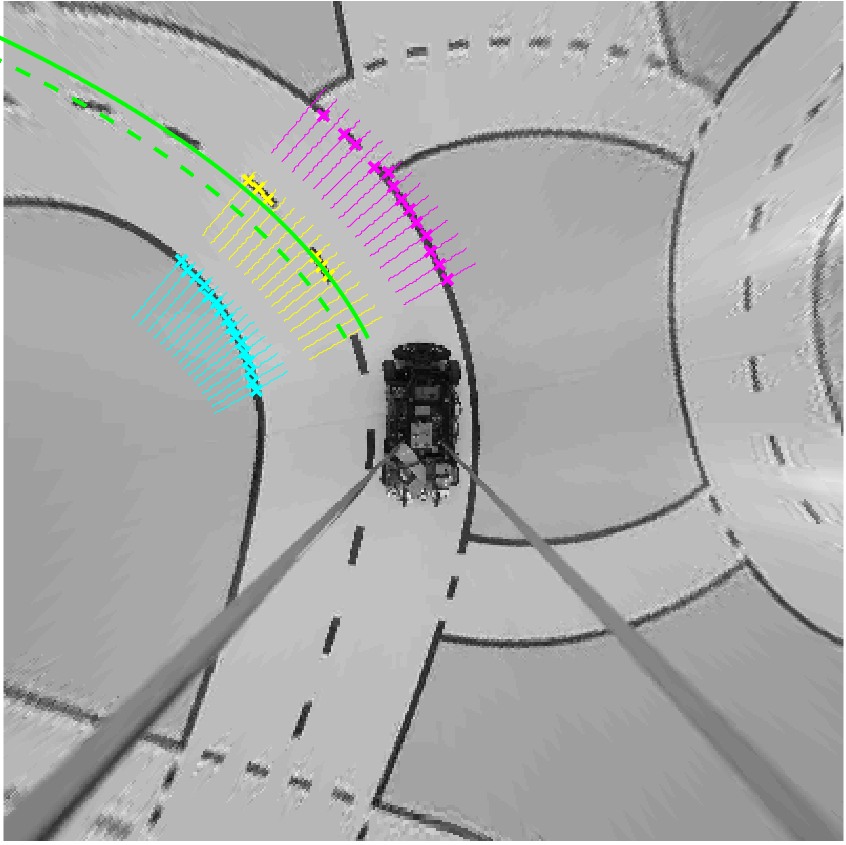
\includegraphics[width=0.45\textwidth]{evaluation_kalman_weggezogen_1}}
	\quad
	\subfloat[][]{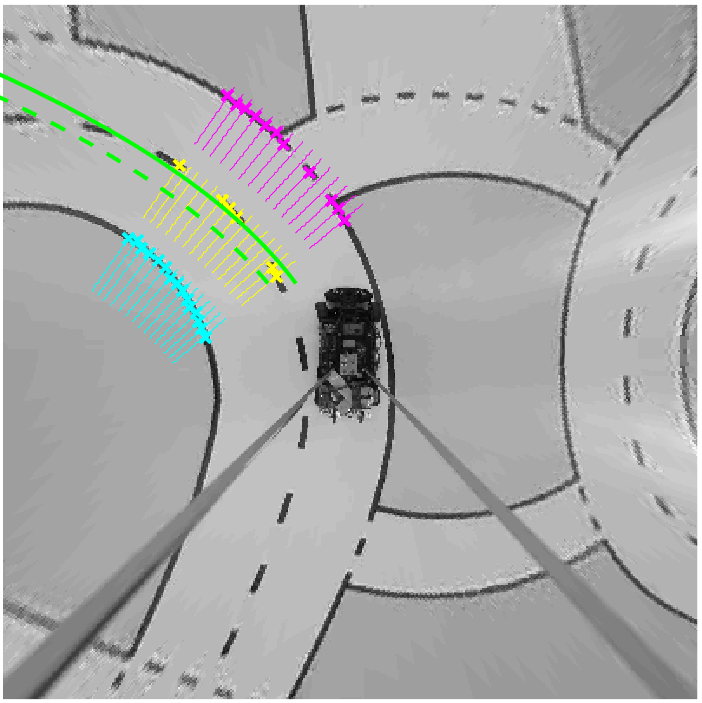
\includegraphics[width=0.45\textwidth]{evaluation_kalman_weggezogen_2}}
	\quad
	\subfloat[][]{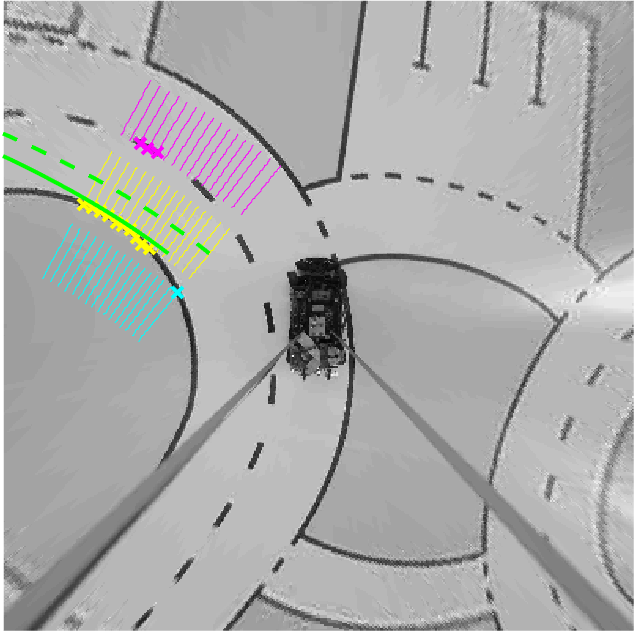
\includegraphics[width=0.45\textwidth]{evaluation_kalman_weggezogen_3}}
	\quad
	\subfloat[][]{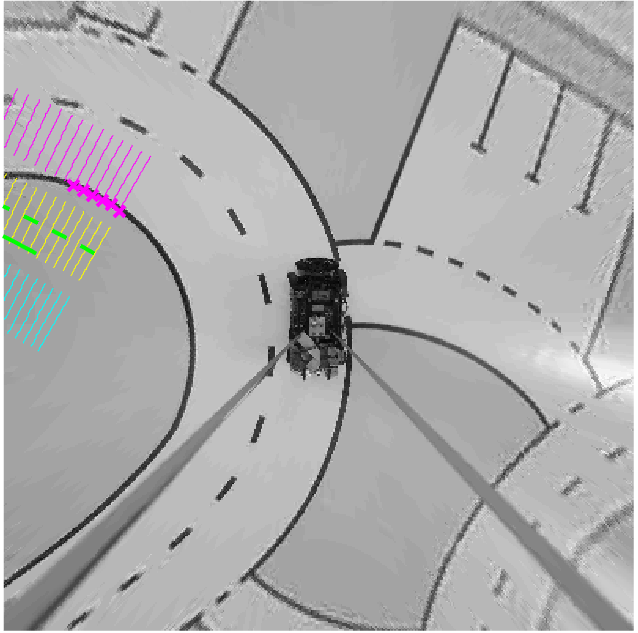
\includegraphics[width=0.45\textwidth]{evaluation_kalman_weggezogen_4}}
	\quad
	\subfloat[][]{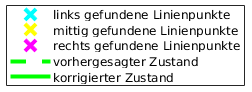
\includegraphics[width=0.45\textwidth]{evaluation_kalman_weggezogen_legende}}
	\caption{\glqq Weglaufen \grqq des Kalmanfilter-Zustands durch ungenügende Vorhersage}
	\label{fig:evaluation:kalman:weggezogen}
\end{figure}

Eine Variante dieses Phänomen zu verhindern, wäre eine Verbesserung des Zustandsraummodells. 
Ein Einbinden des Lenkwinkels, der Winkelgeschwindigkeit oder Orientierung des Fahrzeugs als Eingang \gls{lat:inputvector} wäre theoretisch möglich. Da der Zusammenhang zwischen diesen Größen und den Elementen des Zustandsvektors \gls{lat:statevector} leider nicht trivial ist und keine Literaturquelle vorliegt, in der ein Zustandsraummodell mit diesen Eingangsgrößen gezeigt ist, wurde jedoch vorerst darauf verzichtet. Oft wird in der Literatur bei Nutzung eines Kalmanfilters zur Fahrspurverfolgung sogar gänzlich von einer Vorhersage abgesehen, d.h. \(\gls{lat:systemmatrix}=\gls{lat:unitmatrix}\) \autocite{limRiverFlowLane2012}.

Eine weitere Möglichkeit zur Verbesserung der Performance des vorgeschlagenen Algorithmus stellt die Erhöhung der Bildrate dar. Hierdurch kann eine ungenaue Vorhersage durch häufige Korrektur ausgeglichen werden. Durch eine noch effizientere Implementierung, Parameteroptimierung sowie eine Verkleinerung der Auflösung und/oder des Bildausschnittes könnte dies erzielt werden. Da der in Passage~\ref{sec:fahrspurerkennung:riverflow} beschriebene Ansatz ohne jegliche Optimierung im jetzigen Testszenario weitaus bessere Ergebnisse lieferte, wurde jedoch keine weitere Verfeinerung dieser Methode vorgenommen.

Einen weiteren signifikanten Nachteil stellt wie in Abschnitt \ref{ssec:evaluation:ransac:probleme} beschrieben die Modellierung der Fahrspur durch ein Polynom 3. Grades \(\gls{y}(\gls{x})\) dar, welches schon eine 90\(^\circ\)-Kurve sehr schlecht approximieren kann, da dessen Anstieg unendlich werden müsste. Die volle Sichtweite des Fahrzeugs kann somit nicht genutzt werden (siehe z.B. Abb.~\ref{fig:evaluation:kalman:weggezogen}).



